%%%%%%%%%%%%%%%%%%%%%%%%%%%%%%%%%%%%%%%%%%%%%%%%%%%%%%%%%%%%%%%%%%%%%%%%%%%%%%%%%%
\begin{frame}[fragile]\frametitle{}
\begin{center}
{\Large Overview of ChatGPT}
\end{center}
\end{frame}

%%%%%%%%%%%%%%%%%%%%%%%%%%%%%%%%%%%%%%%%%%%%%%%%%%%%%%%%%%%
\begin{frame}[fragile]\frametitle{What is ChatGPT?}


\begin{itemize}
\item A Chatbot
\item A language model, that takes 'prompt' from user and generates a response.
\item Built by OpenAI and released in Nov 2022
\item Got 1m users in 5 days  (Insta 2.5 months, Spotify 5m, Facebook 10m, Netflix 3.5yrs)
\end{itemize}	 

\begin{itemize}
\item Link: https://chat.openai.com/chat
\item Details: https://openai.com/blog/chatgpt/
\end{itemize}	 

\begin{center}
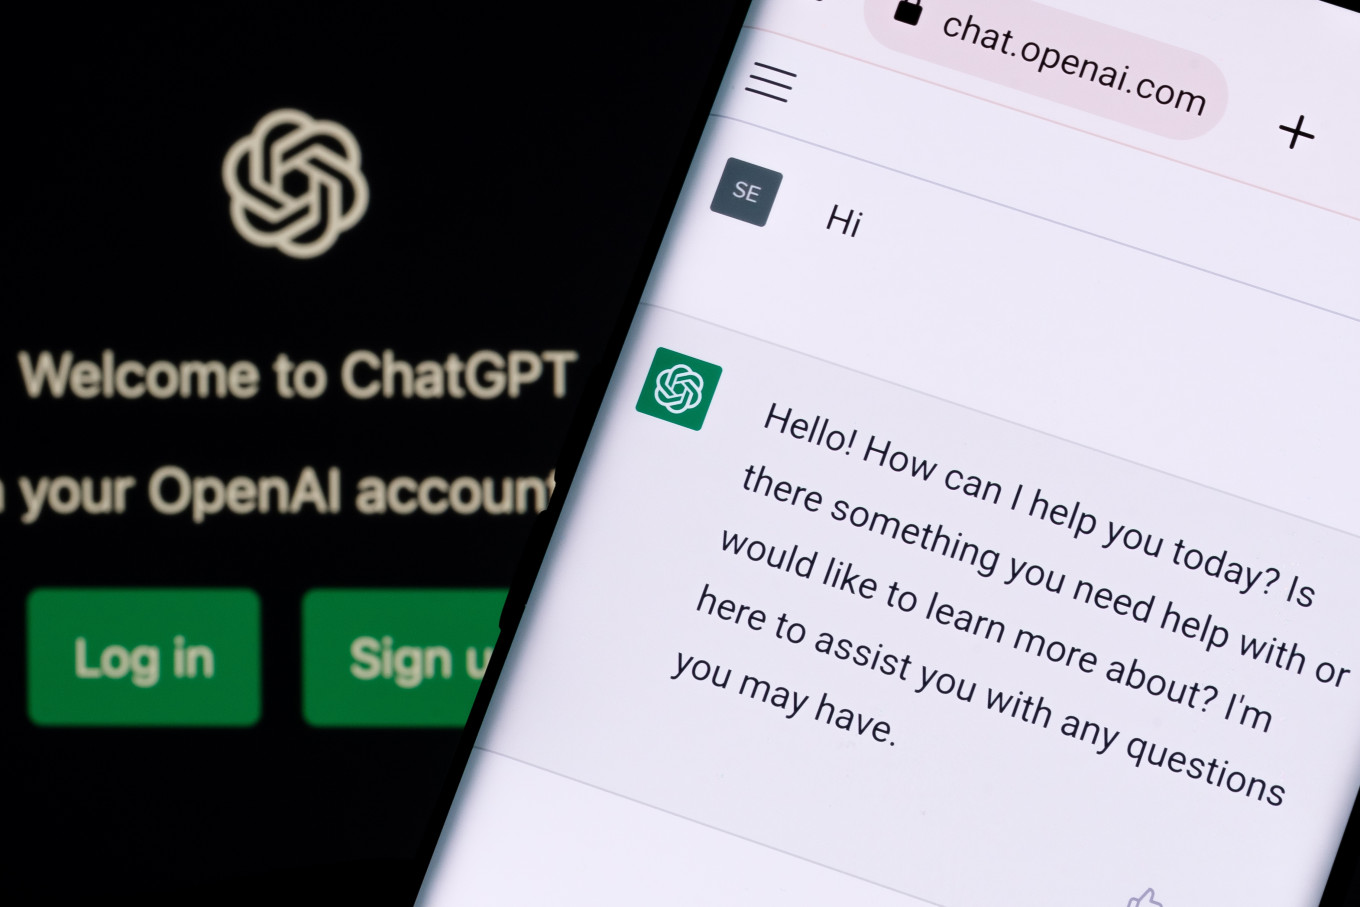
\includegraphics[width=0.5\linewidth,keepaspectratio]{chatgpt33}
\end{center}		
		
{\tiny (Ref: OpenAI, creator of ChatGPT, casts spell on Microsoft
- The Jakarta Post}
			
			
\end{frame}

% %%%%%%%%%%%%%%%%%%%%%%%%%%%%%%%%%%%%%%%%%%%%%%%%%%%%%%%%%%%
% \begin{frame}[fragile]\frametitle{What is ChatGPT?}

% ChatGPT is powered by a Large Language Model (GPT-3.5) optimized for 
% dialogue, developed by OpenAI

% \begin{itemize}
% \item Link: https://chat.openai.com/chat
% \item Details: https://openai.com/blog/chatgpt/
% \end{itemize}	 

% \begin{center}
% 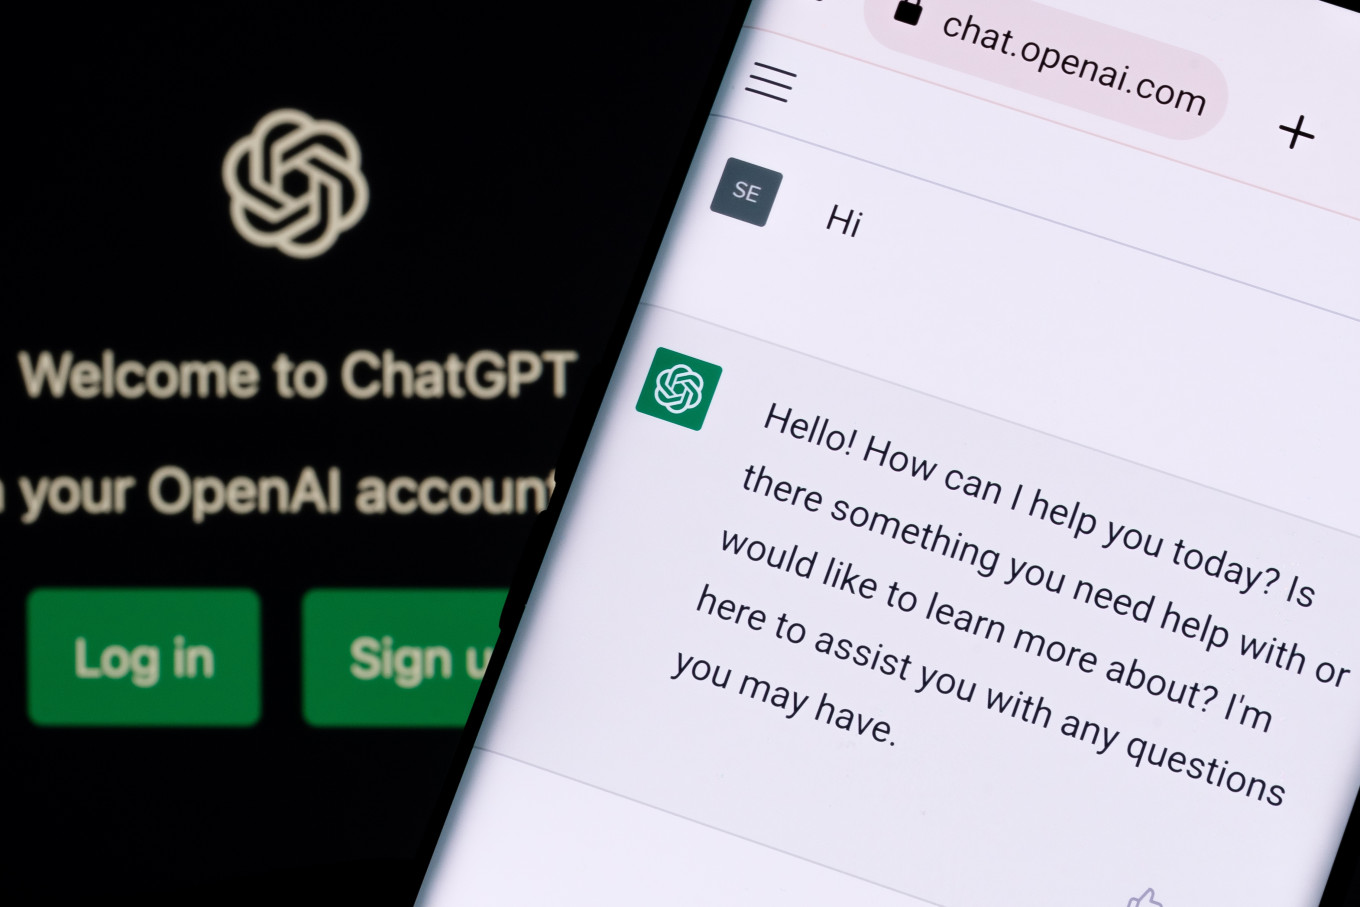
\includegraphics[width=0.6\linewidth,keepaspectratio]{chatgpt33}
% \end{center}		
		
% {\tiny (Ref: OpenAI, creator of ChatGPT, casts spell on Microsoft
% - The Jakarta Post}

% \end{frame}

%%%%%%%%%%%%%%%%%%%%%%%%%%%%%%%%%%%%%%%%%%%%%%%%%%%%%%%%%%%
\begin{frame}[fragile]\frametitle{What is a Language Models?}

\begin{itemize}
\item While typing SMS, have you seen it suggests next word?
\item While typing email, have you seen next few words are suggested?
\item How does it suggest? (suggestions are not random, right?)
\item In the past, for ``Lets go for a \ldots', if you have typed 'coffee' 15 times, 'movie' say 4 times, then it learns that. Machine/Statistical Learning.
\item Next time, when you type ``Lets go for a '', what will be suggested? why?
\item This is called Language Model. Predicting the next word. When done continuously, one after other, it spits sentence, called Generative Model.
\end{itemize}	

\begin{center}
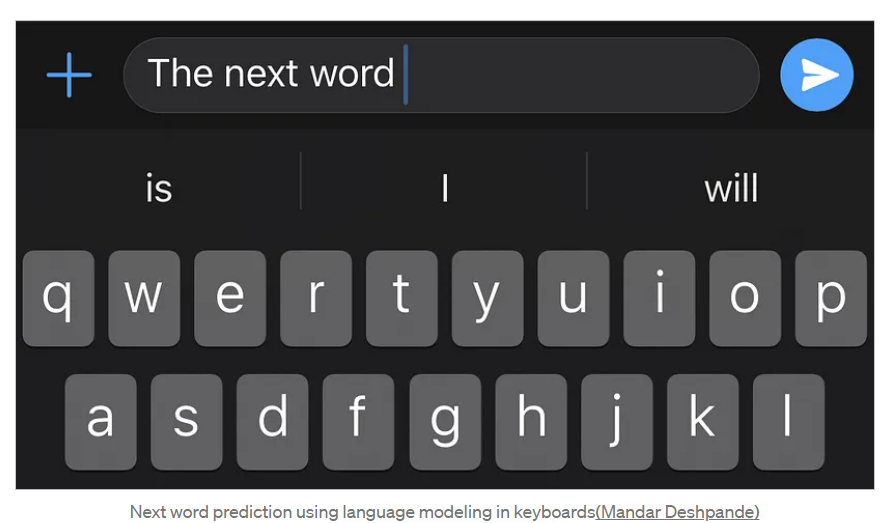
\includegraphics[width=0.6\linewidth,keepaspectratio]{chatgpt34}
\end{center}		

\end{frame}

% %%%%%%%%%%%%%%%%%%%%%%%%%%%%%%%%%%%%%%%%%%%%%%%%%%%%%%%%%%%
% \begin{frame}[fragile]\frametitle{Evolution of Language Models}

% Language Models can be statistical (frequency based) or Machine/Deep Learning (supervised) based. Simple to complex.

% \begin{center}
% 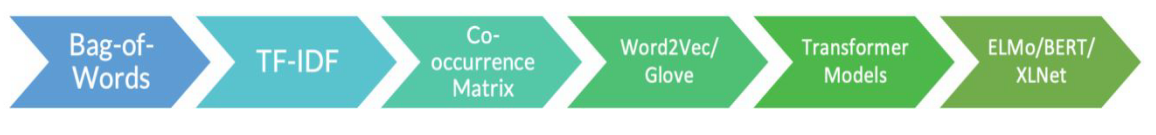
\includegraphics[width=\linewidth,keepaspectratio]{chatgpt30}
% \end{center}				
% {\tiny (Ref: Analytics Vidhya https://editor.analyticsvidhya.com/uploads/59483evolution\_of\_NLP.png)}

% \end{frame}

%%%%%%%%%%%%%%%%%%%%%%%%%%%%%%%%%%%%%%%%%%%%%%%%%%%%%%%%%%%
\begin{frame}[fragile]\frametitle{Large Language Models - Comparison}

\begin{center}
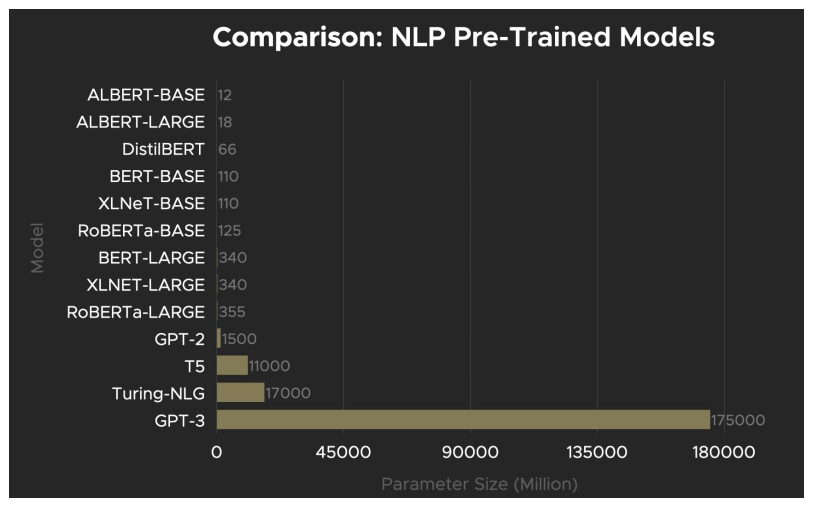
\includegraphics[width=\linewidth,keepaspectratio]{chatgpt31}
\end{center}				
{\tiny (Ref: Deus.ai https://www.deus.ai/post/gpt-3-what-is-all-the-excitement-about)}

\end{frame}



% %%%%%%%%%%%%%%%%%%%%%%%%%%%%%%%%%%%%%%%%%%%%%%%%%%%%%%%%%%%
% \begin{frame}[fragile]\frametitle{What is ChatGPT?}


% \begin{itemize}
% \item GPT based
% \item Trained on large amount of data
% \item Uses Supervised Learning and Reinforcement Learning.
% \item Gives answers like a human
% \item Can ask Follow-up questions and even admit mistakes.
% \end{itemize}	 

% \end{frame}


%%%%%%%%%%%%%%%%%%%%%%%%%%%%%%%%%%%%%%%%%%%%%%%%%%%%%%%%%%%
\begin{frame}[fragile]\frametitle{Open AI: Who are these guys?}


\begin{itemize}
\item San Francisco-based artificial intelligence company
\item Famous for its well-known DALL-E, generates images from prompts.
% \item OpenAI Inc. is the non-profit parent company of the for-profit OpenAI LP.
\item Initially supported by Elon Musk
\item The CEO is Sam Altman, who previously was president of Y Combinator.
\item Microsoft is a partner and investor.
\item Mission: To ensure that artificial general intelligence benefits all of humanity. Prevent misuse of AI
\end{itemize}	 

\begin{center}
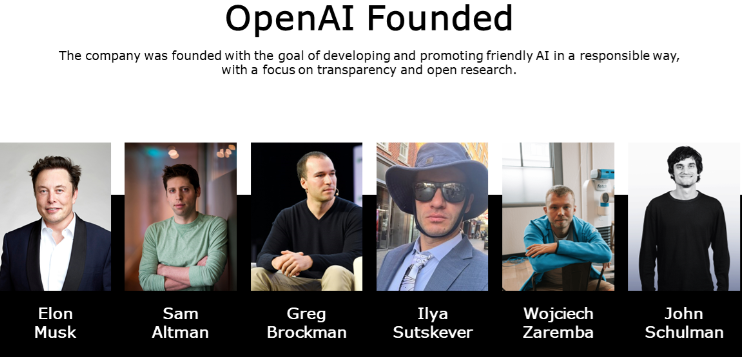
\includegraphics[width=0.8\linewidth,keepaspectratio]{chatgpt25}
\end{center}				
{\tiny (Ref: https://www.slideegg.com/open-ai-chat-gpt)}


\end{frame}

% %%%%%%%%%%%%%%%%%%%%%%%%%%%%%%%%%%%%%%%%%%%%%%%%%%%%%%%%%%%
% \begin{frame}[fragile]\frametitle{How to Use ChatGPT?}


% \begin{center}
% 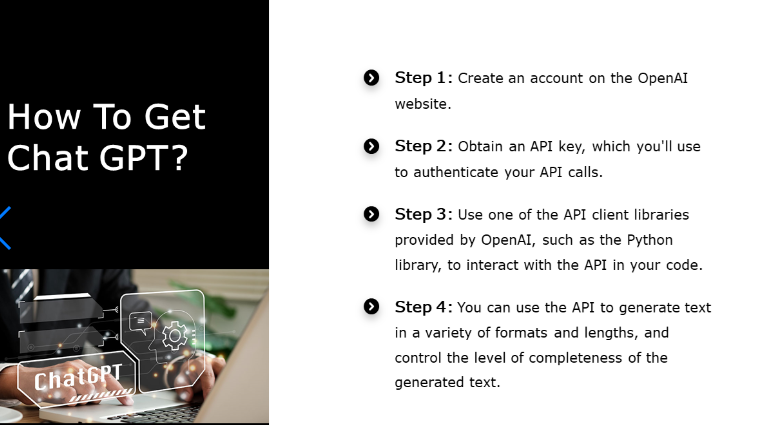
\includegraphics[width=\linewidth,keepaspectratio]{chatgpt26}
% \end{center}				
% {\tiny (Ref: https://www.slideegg.com/open-ai-chat-gpt)}


% \end{frame}


% %%%%%%%%%%%%%%%%%%%%%%%%%%%%%%%%%%%%%%%%%%%%%%%%%%%%%%%%%%%
% \begin{frame}[fragile]\frametitle{GPTs Series}


% \begin{itemize}
% \item GPT + Generative Pre-trained Transformers
% \item GPT-1, GPT-2 and GPT-3 are similar in terms of architecture 
% \item Differ on the data and the number of transformer blocks with the number of incoming tokens.   
% \item GPT-1 : 12 blocks, encoded using a Byte pair encoding, 512 tokens: 117 million parameters 
% \item GPT-2 : 48 blocks, 1024 tokens: 1.5 billion parameters 
% \item GPT-3 : 96 blocks, 2048 tokens: 175 billion parameters 
% \end{itemize}	 

% \end{frame}

%%%%%%%%%%%%%%%%%%%%%%%%%%%%%%%%%%%%%%%%%%%%%%%%%%%%%%%%%%%
\begin{frame}[fragile]\frametitle{GPTs Training}

GPT: Generative Pre-trained Transformers

\begin{itemize}
% \item GPT-1 is trained in a self-supervised manner (learn to predict the next word in text data) and fine-tuned in a supervised learning manner. 
% \item GPT-2 is trained in a fully self supervised way, focusing on zero-shot transfer
% \item  GPT-3 is pre-trained in a self supervised manner exploring a bit more the few-shots fine-tuning.
\item GPT-1 is pre-trained on the BooksCorpus dataset, containing ~7000 books amounting to ~5GB of data
\item GPT-2 is pre-trained using the WebText dataset which is a more diverse set of internet data containing ~8M documents for about ~40 GB of data
\item GPT-3 uses an expanded version of the WebText dataset, two internet-based books corpora that are not disclosed and the English-language Wikipedia which constituted ~600 GB of data
\end{itemize}	 

\end{frame}

%%%%%%%%%%%%%%%%%%%%%%%%%%%%%%%%%%%%%%%%%%%%%%%%%%%%%%%%%%%
\begin{frame}[fragile]\frametitle{GPT3 vs ChatGPT}


\begin{center}
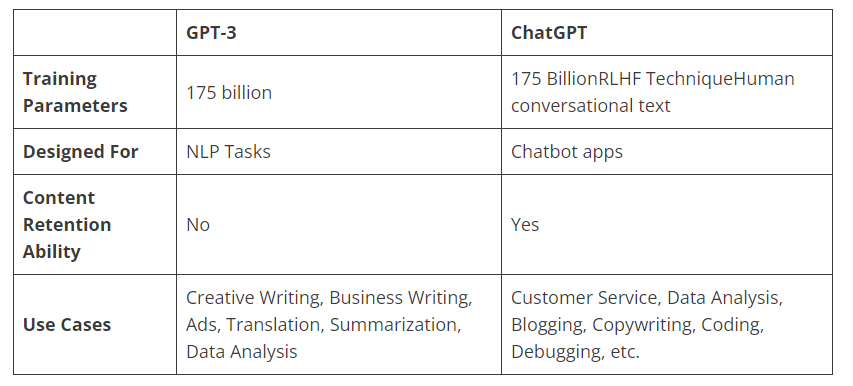
\includegraphics[width=0.8\linewidth,keepaspectratio]{chatgpt27}
\end{center}		

\tiny{(Ref:ChatGPT Explained: Complete A-Z Guide - Kripesh Adwani)}
\end{frame}

% %%%%%%%%%%%%%%%%%%%%%%%%%%%%%%%%%%%%%%%%%%%%%%%%%%%%%%%%%%%
% \begin{frame}[fragile]\frametitle{GPT Training: Overview}


% Task: predicting next word

% \begin{center}
% 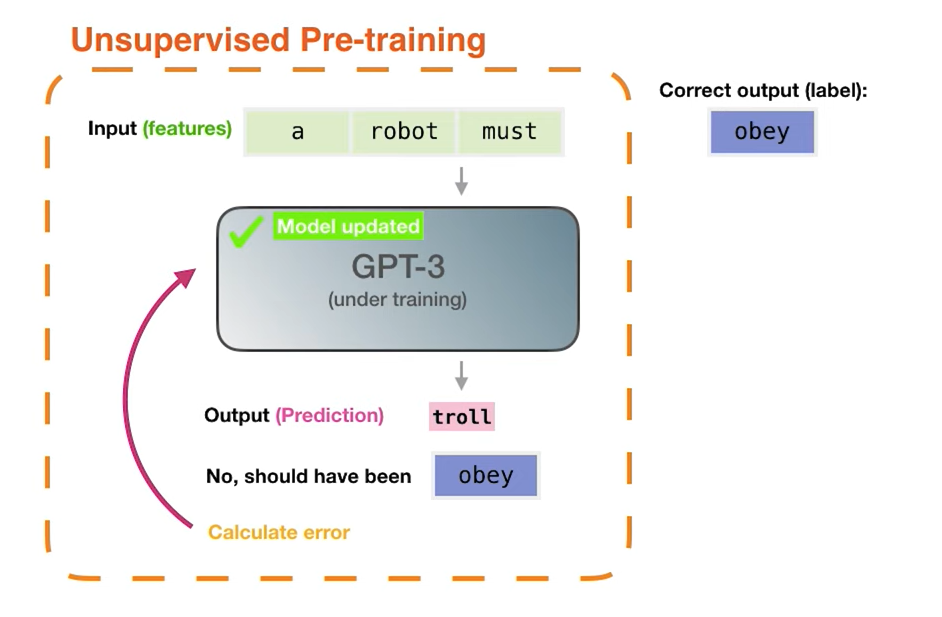
\includegraphics[width=0.8\linewidth,keepaspectratio]{chatgpt13}
% \end{center}		


% {\tiny (Ref: How GPT3 Works - Easily Explained with Animations - Jay Alammar)}

% \end{frame}

% %%%%%%%%%%%%%%%%%%%%%%%%%%%%%%%%%%%%%%%%%%%%%%%%%%%%%%%%%%%
% \begin{frame}[fragile]\frametitle{GPT Inferencing: Overview}


% GPT being a decoder only model, takes words vectors (does this conversion internally), then through set of Decoder blocks, to spit out the next word one by one

% \begin{center}
% 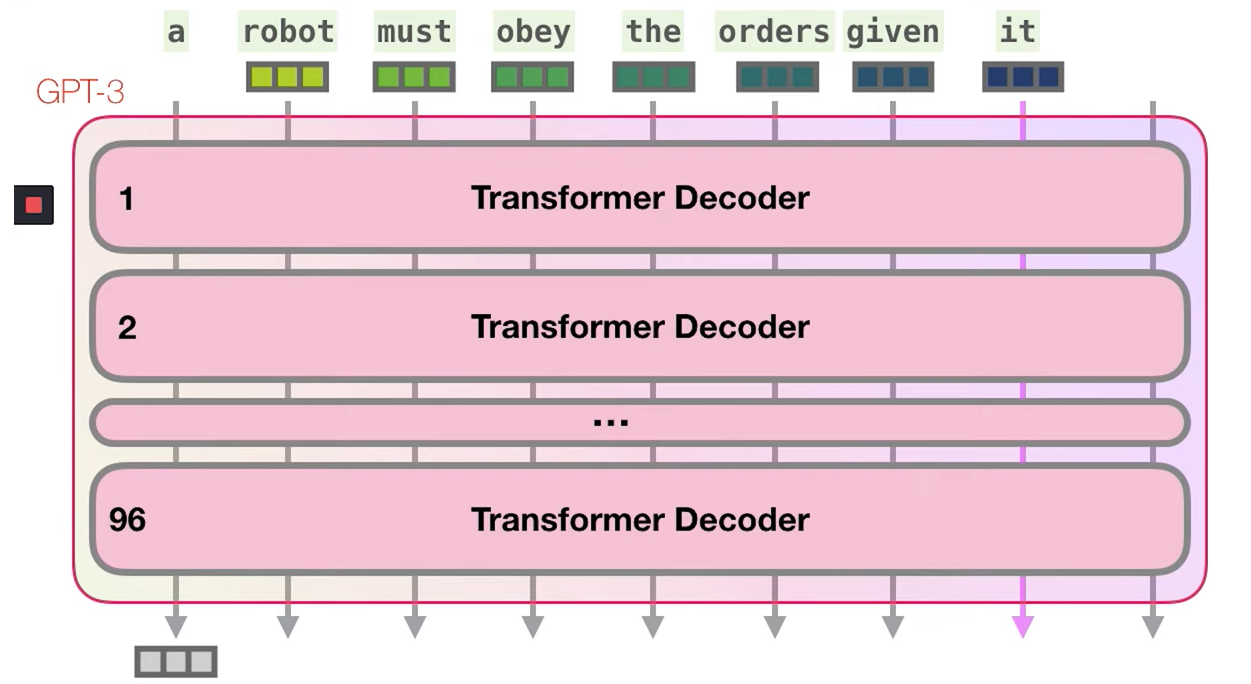
\includegraphics[width=0.8\linewidth,keepaspectratio]{chatgpt14}
% \end{center}		


% {\tiny (Ref: How GPT3 Works - Easily Explained with Animations - Jay Alammar)}

% \end{frame}

% %%%%%%%%%%%%%%%%%%%%%%%%%%%%%%%%%%%%%%%%%%%%%%%%%%%%%%%%%%%
% \begin{frame}[fragile]\frametitle{Misalignment Issue}


% \begin{itemize}
% \item GPT-3 was trained to predict the next word. Not much of context there.
% \item Introducing prompting : provide with certain samples and context

% \end{itemize}	 

			% \begin{center}
			% 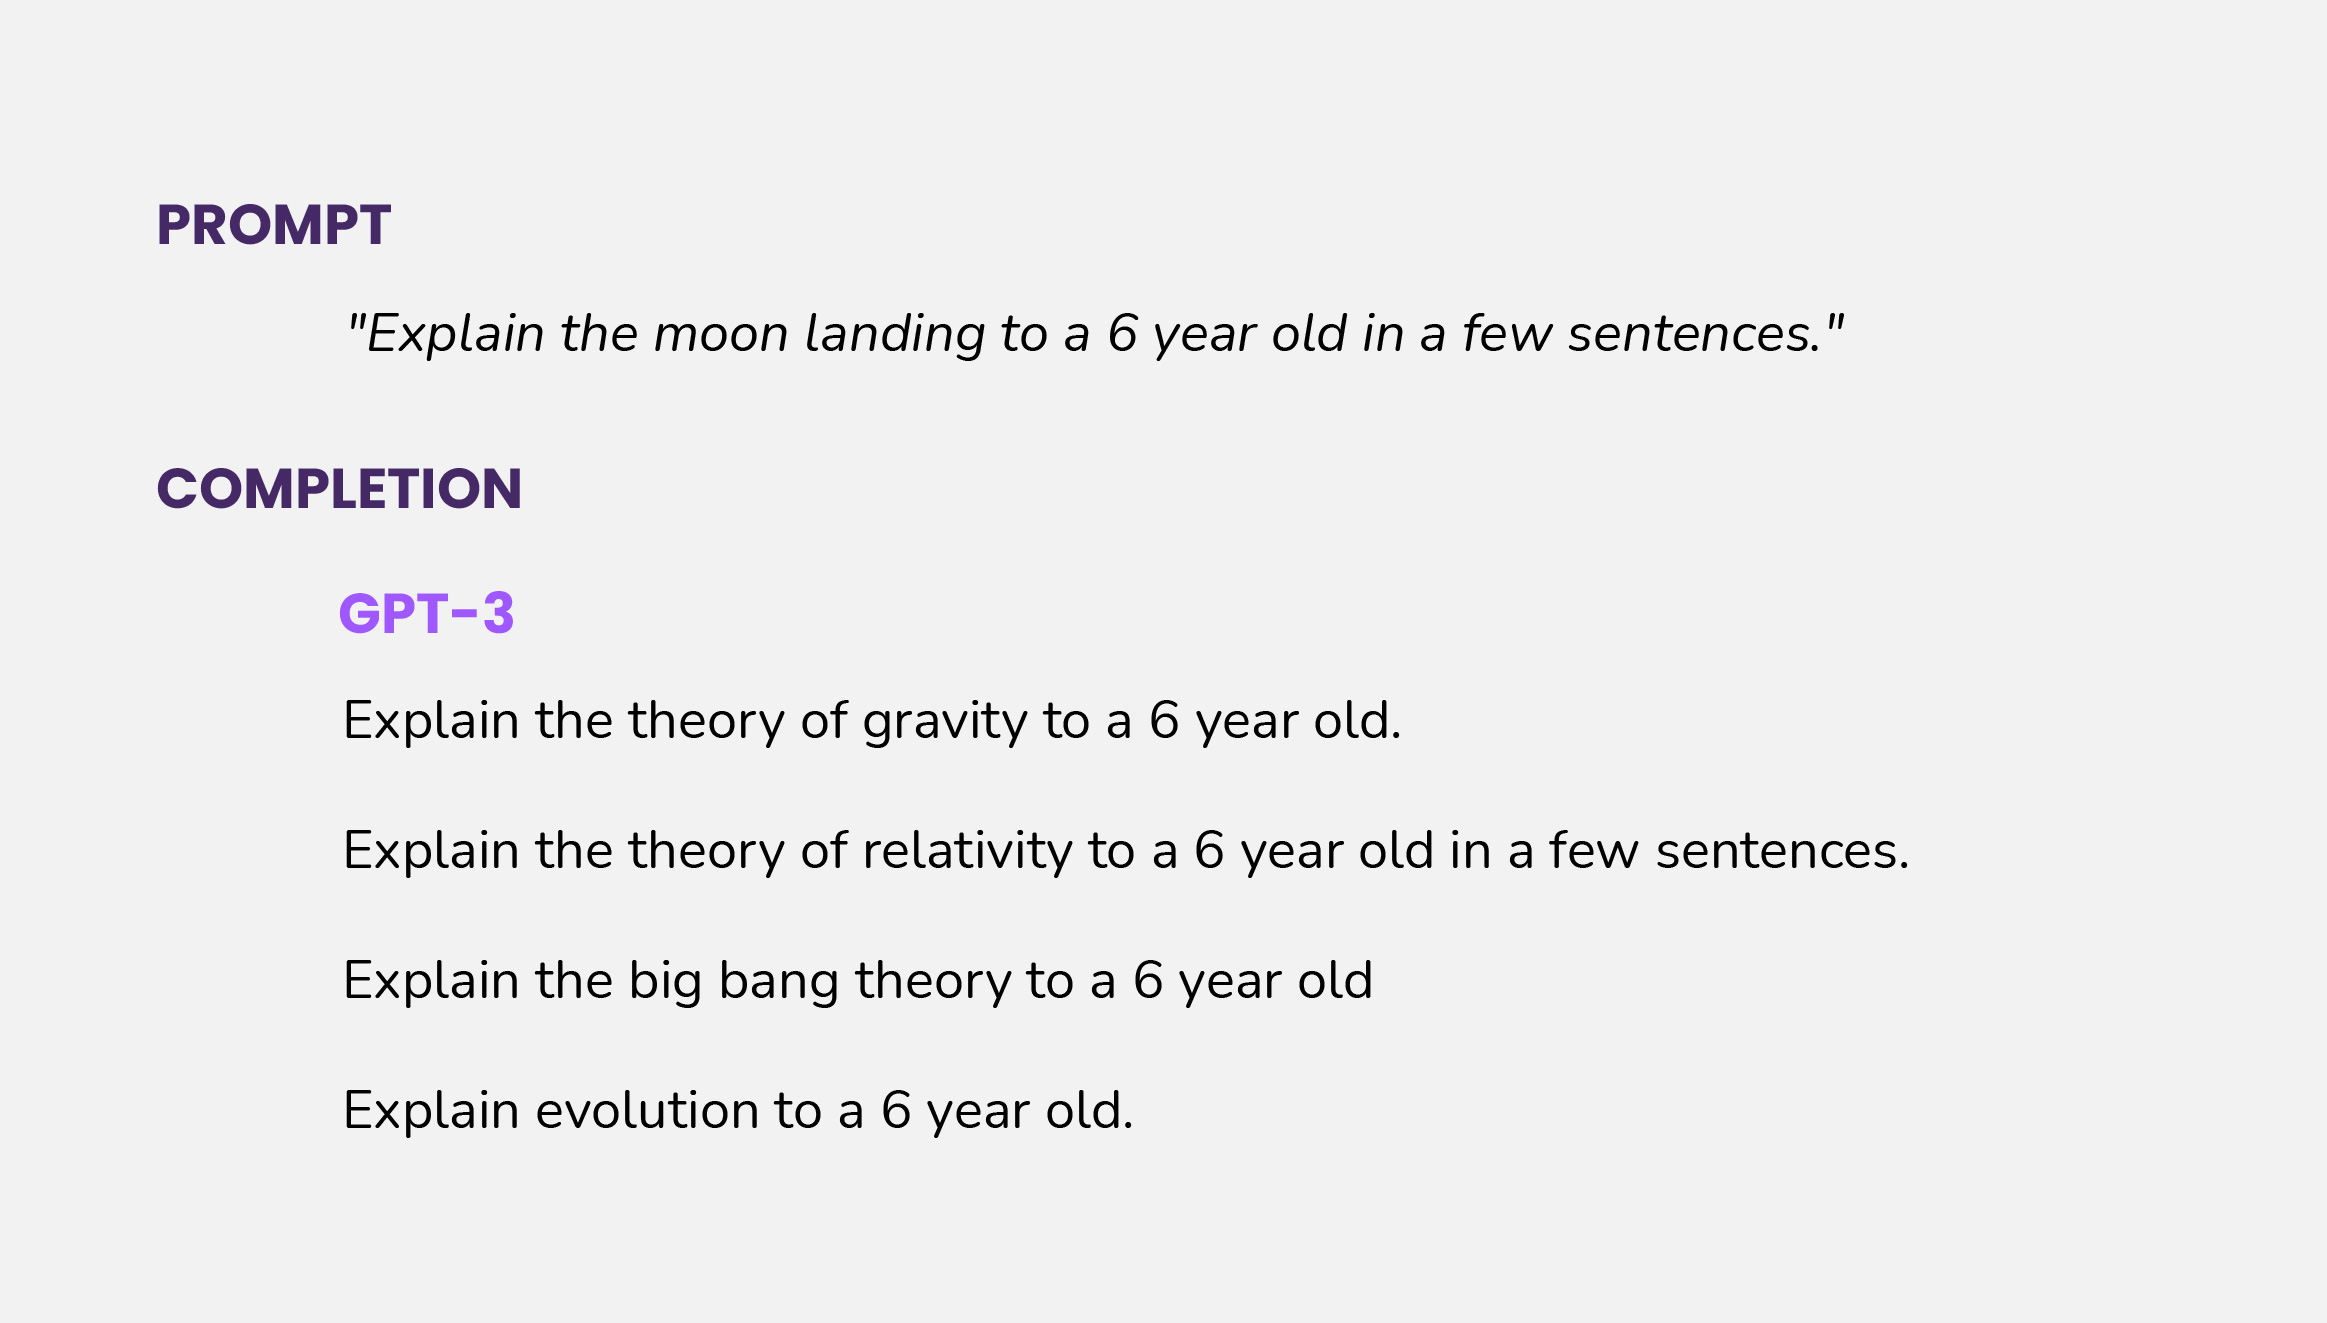
\includegraphics[width=0.6\linewidth,keepaspectratio]{chatgpt2}
			
			% {\tiny "Example of misalignment between text to be predicted and final use"}
			% \end{center}		
			
			
			% {\tiny (Ref: ChatGPT: training process, advantages, and limitations - By Sergio Soage, Machine Learning Engineer at Aivo)}
			
% \end{frame}

% %%%%%%%%%%%%%%%%%%%%%%%%%%%%%%%%%%%%%%%%%%%%%%%%%%%%%%%%%%%
% \begin{frame}[fragile]\frametitle{Curated Training Data}


% \begin{itemize}
% \item To fix this misalignment, humans must be involved in teaching GPT, and in this way, GPT will be able to generate better questions as it evolves.
% \item Reinforcement Learning based on Human Input (rewards if aligns) was leveraged.
% \end{itemize}	 

% \begin{center}
% 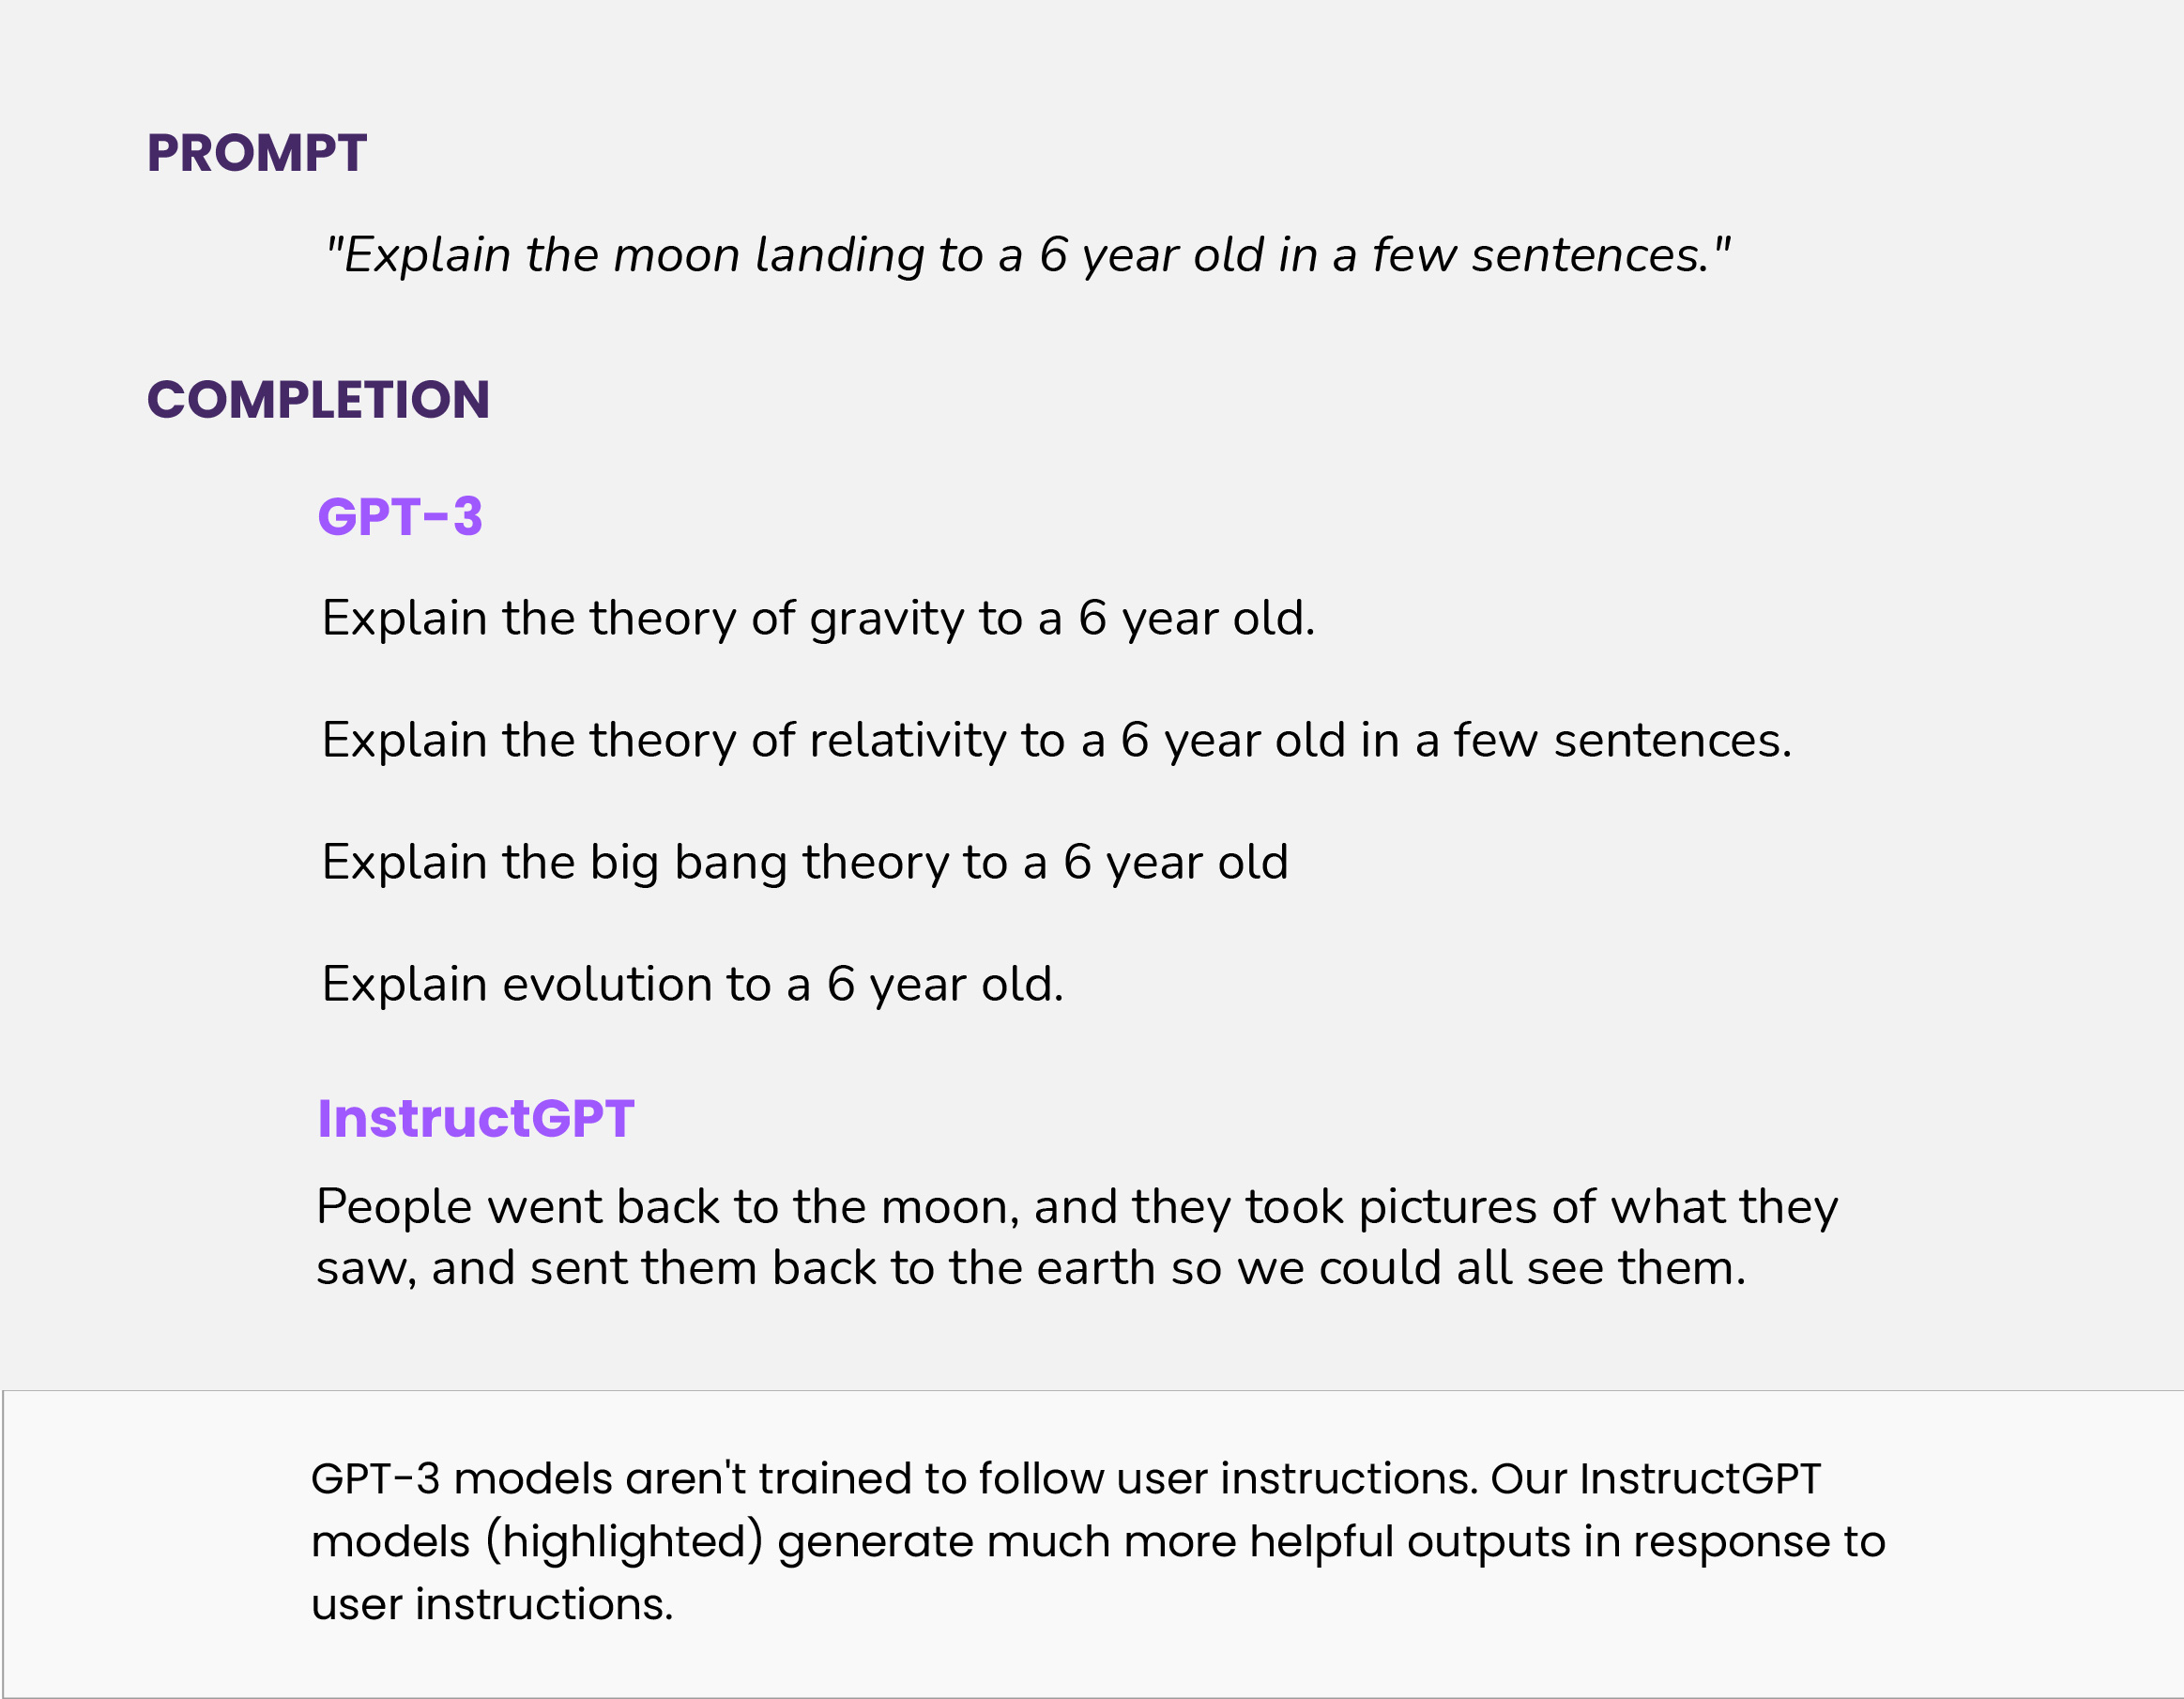
\includegraphics[width=0.6\linewidth,keepaspectratio]{chatgpt3}

% \end{center}		

% {\tiny (Ref: ChatGPT: training process, advantages, and limitations - By Sergio Soage, Machine Learning Engineer at Aivo)}
			
% \end{frame}


% %%%%%%%%%%%%%%%%%%%%%%%%%%%%%%%%%%%%%%%%%%%%%%%%%%%%%%%%%%%
% \begin{frame}[fragile]\frametitle{Prerequisites: What is Reinforcement Learning (RL)?}


% \begin{itemize}
% \item RL is a method of achieving a goal via rewards. Find best path to get maximum points (game below)
% \item Agent: Makes the moves
% \item Reward: Positive or Negative (as shown)
% \item State: Current position, location.
% \item Action: Move done by the Agent
% \item Policy: Sequence of Actions that Agent takes to achieve the goal, say, Down-Down-Right-Right-Right (reward 6)..there could be other paths and one(or more) of then can be the best.
% \end{itemize}	 


% \begin{center}
% 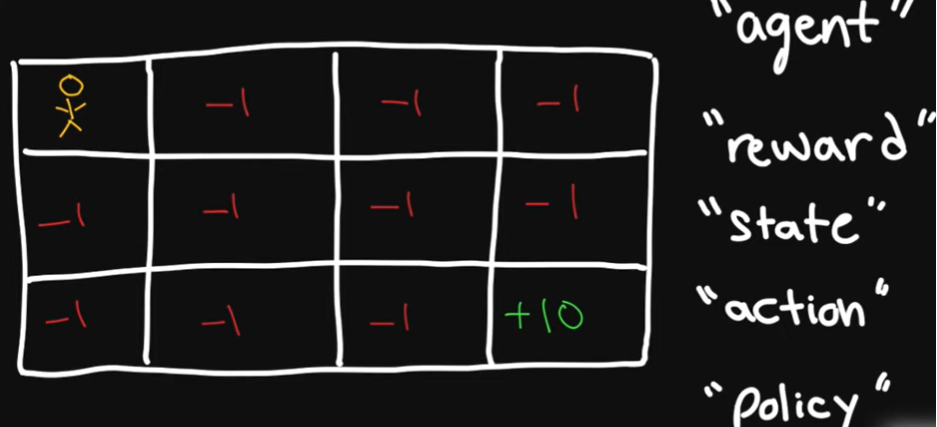
\includegraphics[width=0.6\linewidth,keepaspectratio]{chatgpt9}
% \end{center}		


% {\tiny (Ref: ChatGPT - Explained! - CodeEmporium)}
% \end{frame}

% %%%%%%%%%%%%%%%%%%%%%%%%%%%%%%%%%%%%%%%%%%%%%%%%%%%%%%%%%%%
% \begin{frame}[fragile]\frametitle{RL in context of ChatGPT}


% \begin{itemize}
% \item Agent: the model, it spits out words
% \item Reward: score at predicting each next word
% \item State: prompt + sentence generated so far
% \item Action: Predicting the next word
% \item Policy: Sequence of words and then total rewards for them.
% \item Manual person can chose between such sequences (or polices) and label which is best. Then PPO can happen to adjust backwardly the reward function.
% \item So, the Reinforcement Learning is used to capture human preferences and reduce misalignment.
% \end{itemize}	 
% \end{frame}

% %%%%%%%%%%%%%%%%%%%%%%%%%%%%%%%%%%%%%%%%%%%%%%%%%%%%%%%%%%%
% \begin{frame}[fragile]\frametitle{Better GPT 3.5}

% \begin{itemize}
% \item ChatGPT is slight deviation to InstructGPT model (GPT 3.5)
% \item InstructGPT Paper: ``Training language models to follow instructions with human feedback''
% \end{itemize}	 

% \begin{center}
% 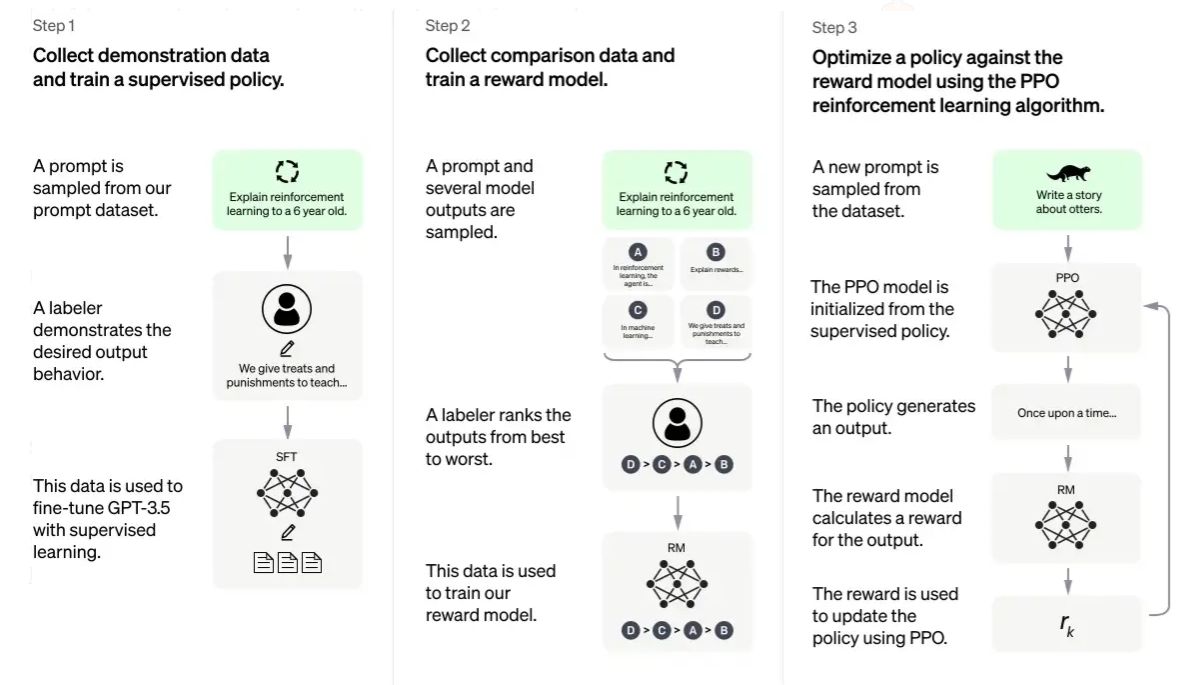
\includegraphics[width=0.8\linewidth,keepaspectratio]{chatgpt1}
% \end{center}		

% \tiny{(Ref: https://openai.com/blog/chatgpt/)}
% \end{frame}

% %%%%%%%%%%%%%%%%%%%%%%%%%%%%%%%%%%%%%%%%%%%%%%%%%%%%%%%%%%%
% \begin{frame}[fragile]\frametitle{How is ChatGPT trained?}
% Step 1

% \begin{itemize}
% \item Have a prompts dataset 
% \item Let human laborer get the correct response for them
% \item Do fine-tuning of GPT 3.5 using this data via supervised learning (SFT). 
% \item Simple but very expensive.
% \end{itemize}	 

			% \begin{center}
			% 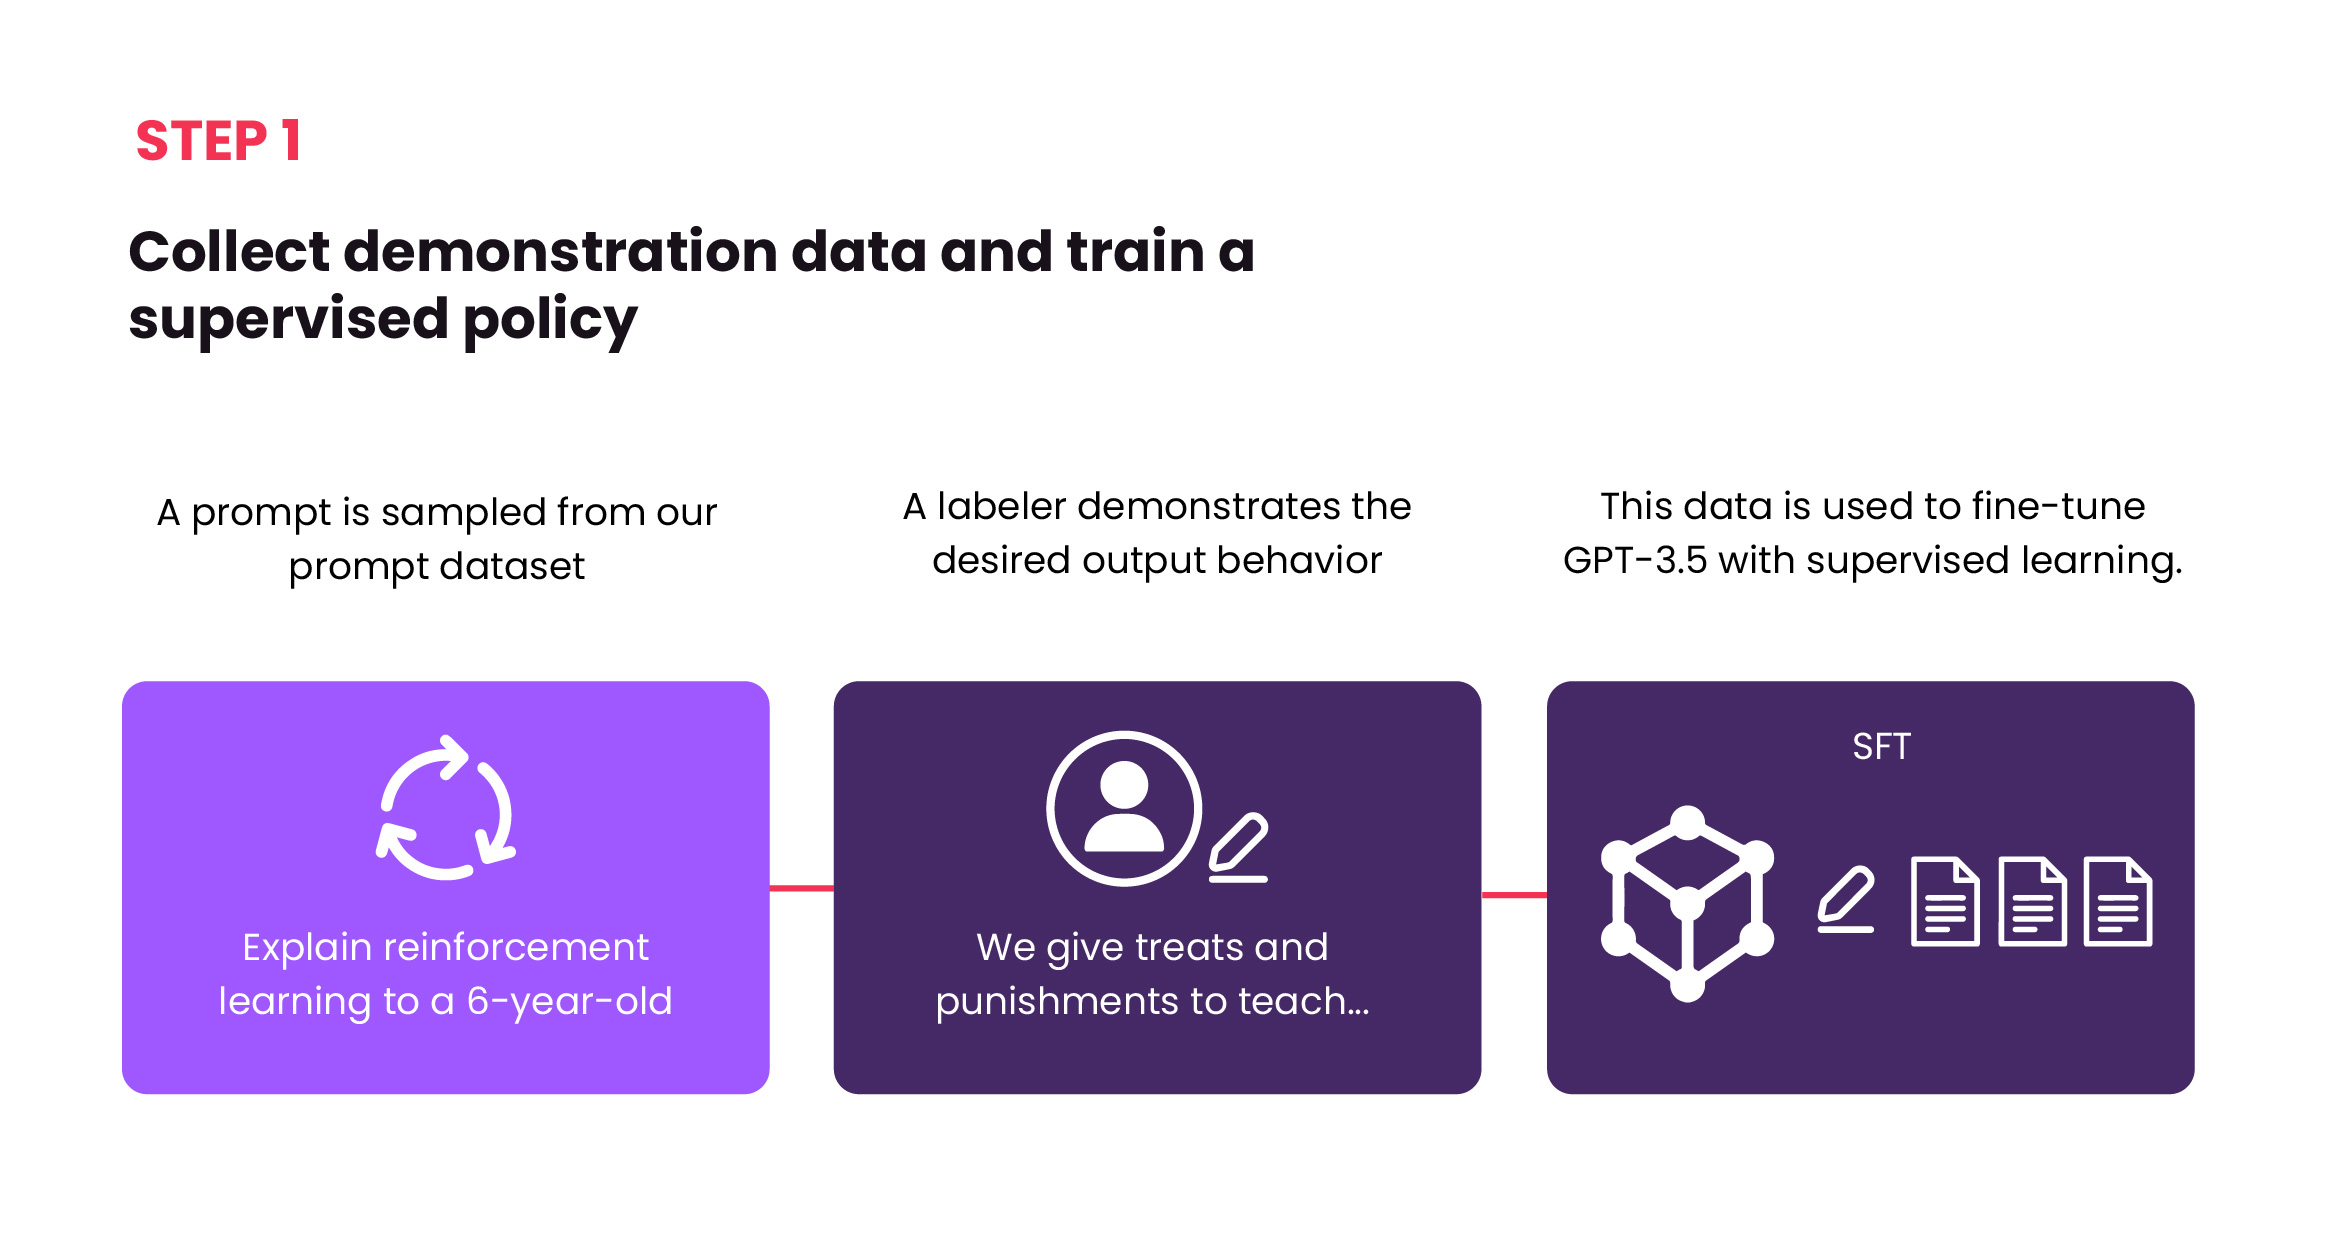
\includegraphics[width=0.8\linewidth,keepaspectratio]{chatgpt4}
			
			% \end{center}		
			
			% {\tiny (Ref: ChatGPT: training process, advantages, and limitations - By Sergio Soage, Machine Learning Engineer at Aivo)}
			
% \end{frame}

% %%%%%%%%%%%%%%%%%%%%%%%%%%%%%%%%%%%%%%%%%%%%%%%%%%%%%%%%%%%
% \begin{frame}[fragile]\frametitle{How is ChatGPT trained?}
% Step 2

% \begin{itemize}
% \item For a prompt, generate multiple responses from the fine-tuned model, one after another.
% \item Human feedback provides a ranking of responses
% \item This data is used to build Rewards Model (RM)
% \end{itemize}	 

			% \begin{center}
			% 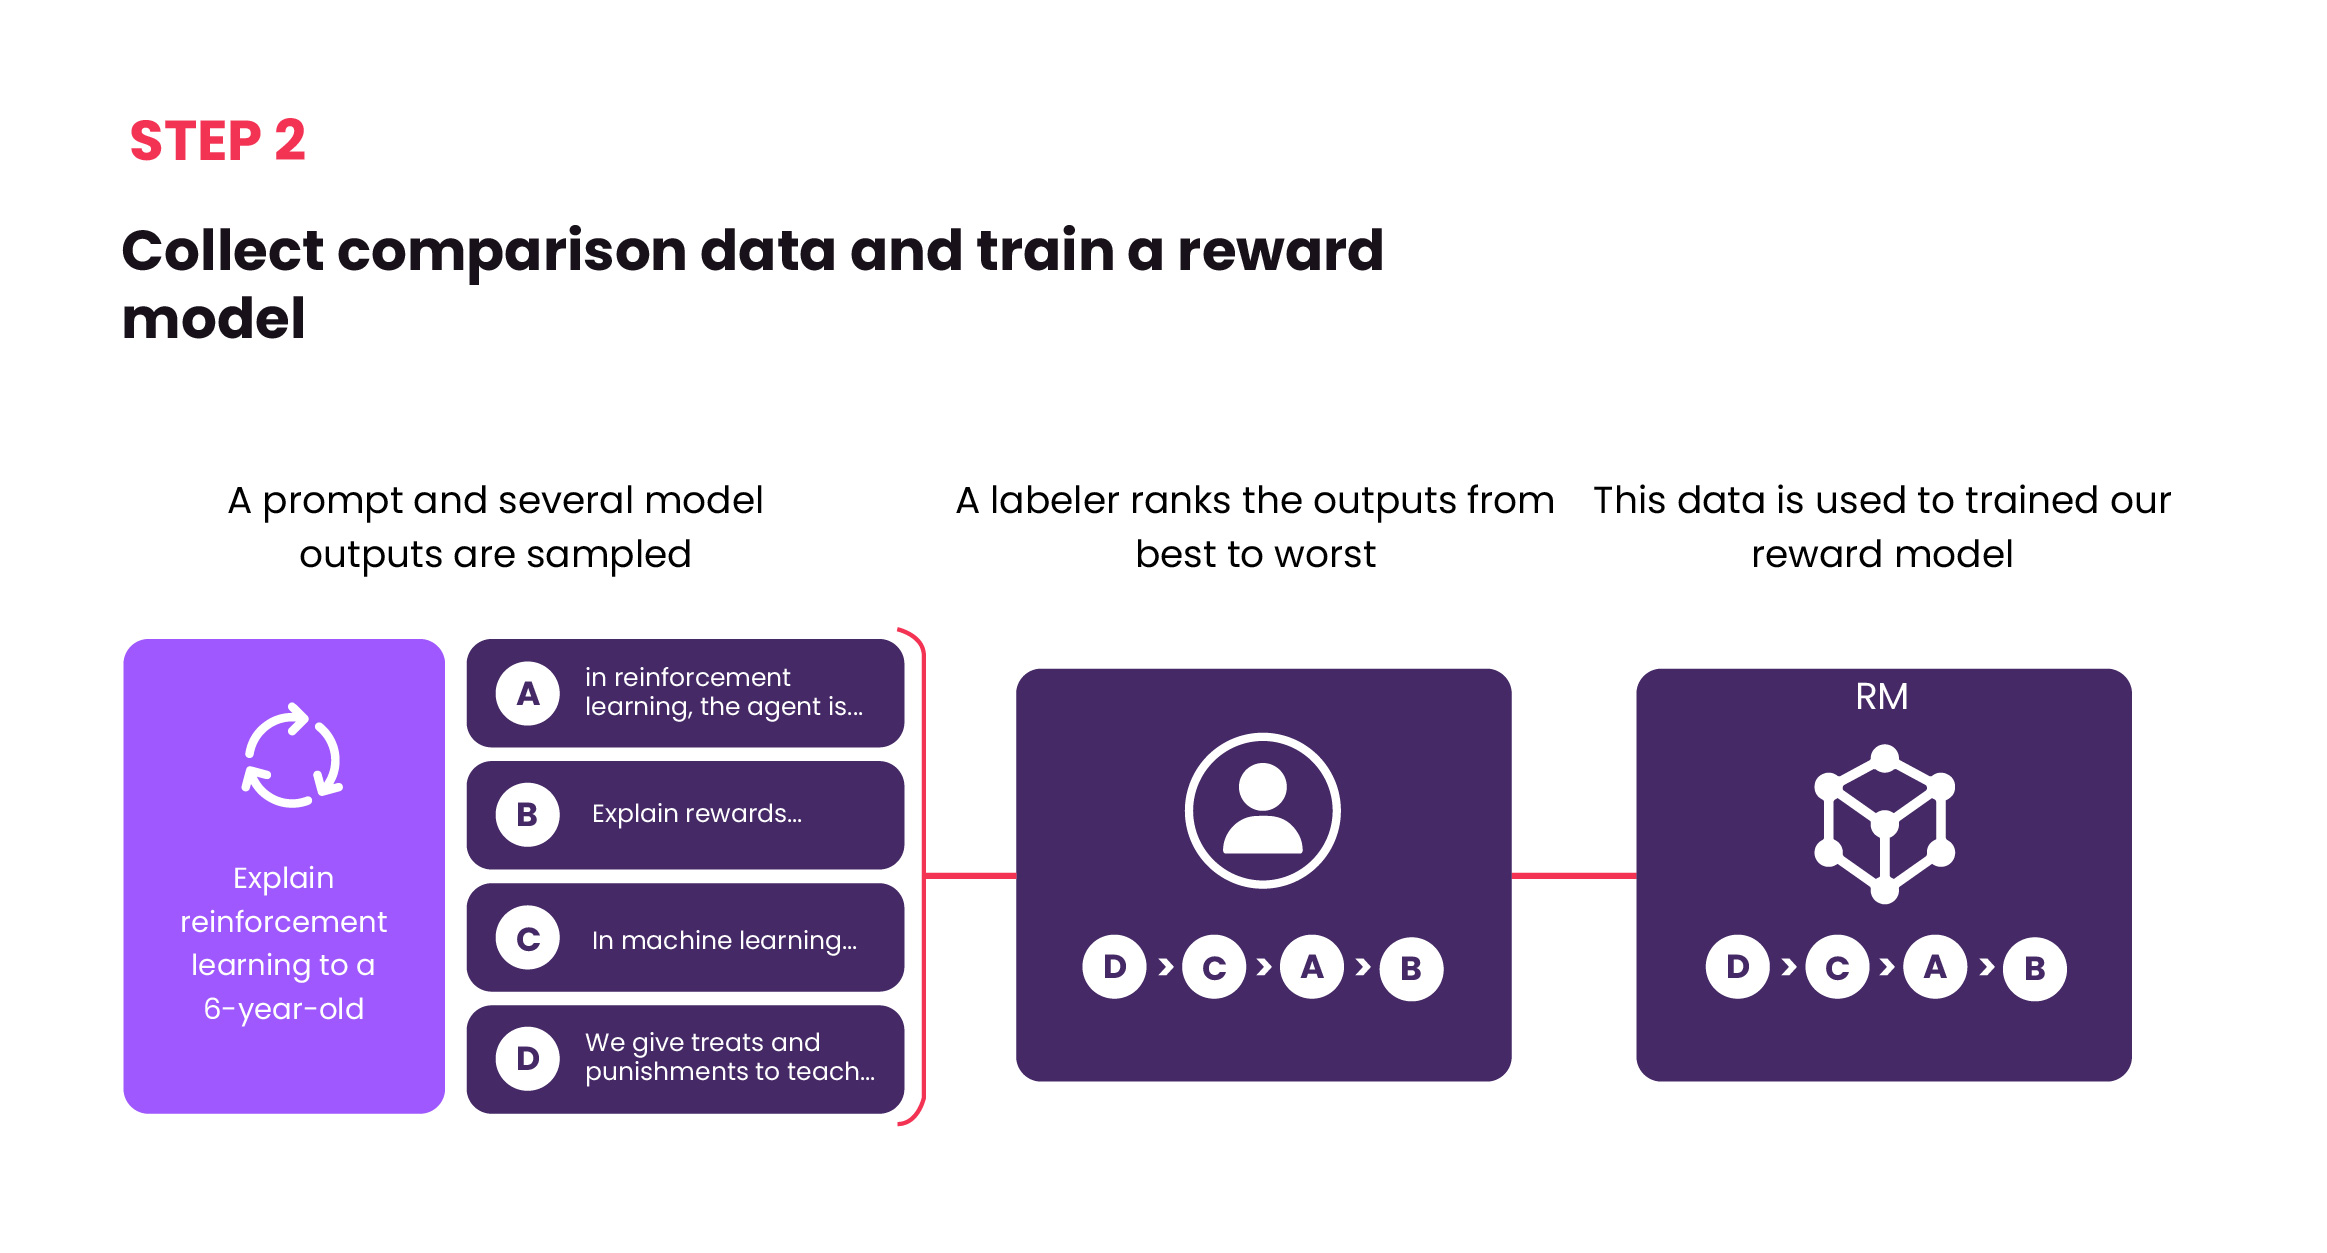
\includegraphics[width=0.8\linewidth,keepaspectratio]{chatgpt5}
			
			% \end{center}		
			
			% {\tiny (Ref: ChatGPT: training process, advantages, and limitations - By Sergio Soage, Machine Learning Engineer at Aivo)}
			
% \end{frame}


% % %%%%%%%%%%%%%%%%%%%%%%%%%%%%%%%%%%%%%%%%%%%%%%%%%%%%%%%%%%%
% % \begin{frame}[fragile]\frametitle{Step 2: Manual Ranking}


			% % \begin{center}
			% % 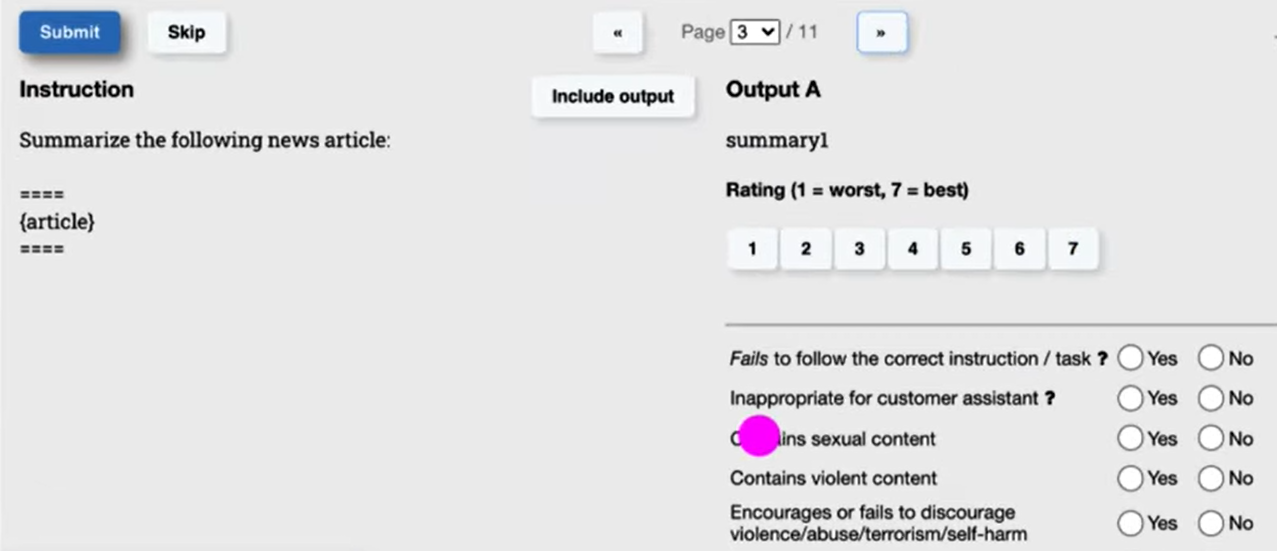
\includegraphics[width=\linewidth,keepaspectratio]{chatgpt10}
			
			% % \end{center}		
			
			% % {\tiny (Ref: ChatGPT - Explained! - CodeEmporium)}
			
% % \end{frame}


% %%%%%%%%%%%%%%%%%%%%%%%%%%%%%%%%%%%%%%%%%%%%%%%%%%%%%%%%%%%
% \begin{frame}[fragile]\frametitle{How is ChatGPT trained?}
% Step 3

% \begin{itemize}
% \item Take unseen prompt. Pass it through Proximal Policy Optimization (PPO) model which has been initialized with SFT. It generates a response (ie inferencing via SFT).
% \item Calculate reward for that response via RM model. This reward is used to update the PPO model (loss function, back-propagation)
% \end{itemize}	 

			% \begin{center}
			% 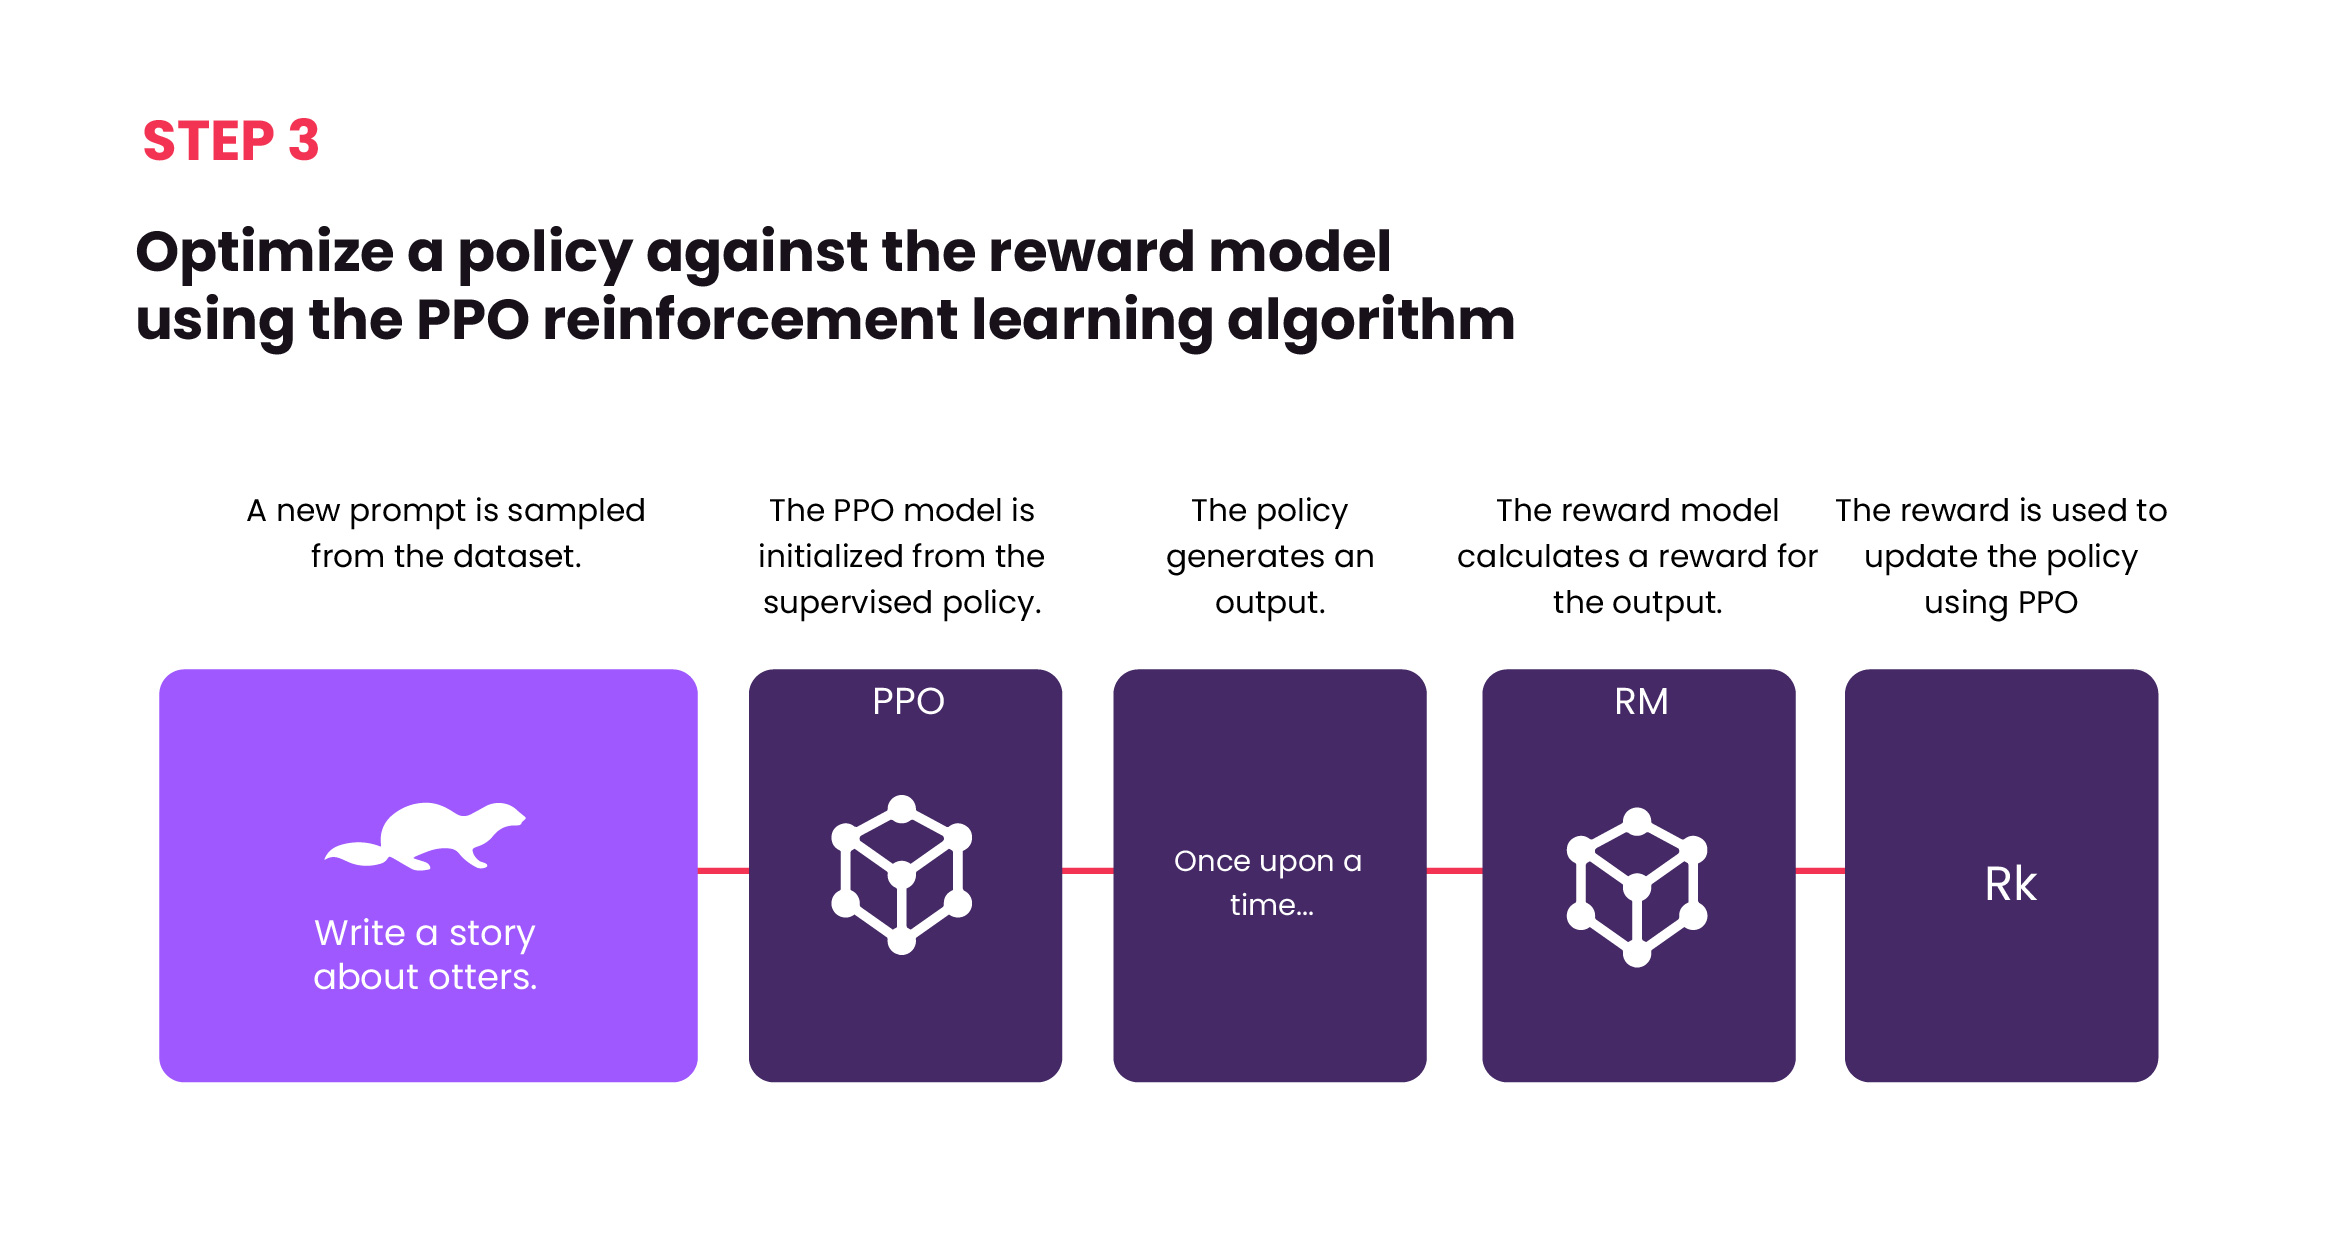
\includegraphics[width=0.8\linewidth,keepaspectratio]{chatgpt6}
			
			% \end{center}		
			
			% {\tiny (Ref: ChatGPT: training process, advantages, and limitations - By Sergio Soage, Machine Learning Engineer at Aivo)}
			
% \end{frame}

% % %%%%%%%%%%%%%%%%%%%%%%%%%%%%%%%%%%%%%%%%%%%%%%%%%%%%%%%%%%%%%%%%%%%%%%%%%%%%%%%%%%
% % \begin{frame}[fragile]\frametitle{As a Python Program?}
% % Pip install openai library, have KEY from your own account and then try various APIs available

			% % \begin{center}
			% % 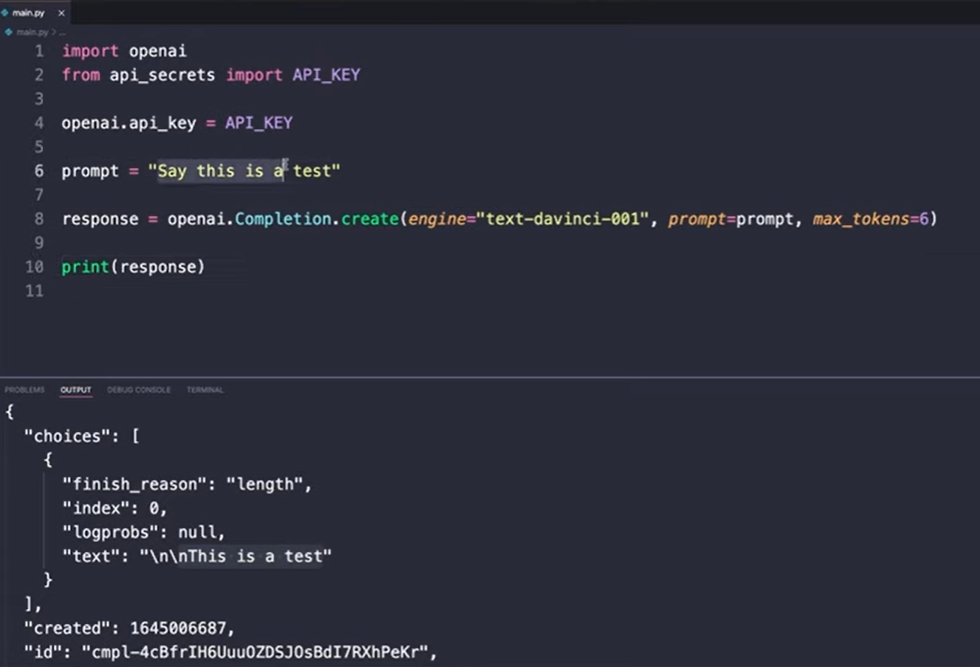
\includegraphics[width=0.8\linewidth,keepaspectratio]{chatgpt12}
			
			% % \end{center}		
			
			% % {\tiny (Ref: Getting Started with OpenAI API and GPT-3 -Assembly AI)}
			

% % \end{frame}


% %%%%%%%%%%%%%%%%%%%%%%%%%%%%%%%%%%%%%%%%%%%%%%%%%%%%%%%%%%%%%%%%%%%%%%%%%%%%%%%%%%
% \begin{frame}[fragile]\frametitle{Completions}

% The most common use case for any LLM is to generate a response from a prompt. In this case, the prompt is “Say this is a test”. OpenAI calls this task “completions”.

% \begin{itemize}
% \item max\_tokens: the maximum number of tokens to generate in the completion
% \item temperature: a value between 0–2. The higher the number, the more spontaneous and random the response will be.
% \item n: the number of completions to generate.
% \item stream: boolean; stream back partial progress.	
% \end{itemize}	 

% {\tiny (Ref: Techy Stuff 1: Notes on Transformers, LLMs, and OpenAI - Bill)}

% \begin{lstlisting}
% response = openai.createCompletion({
  % model="text-davinci-003",
  % prompt="Say this is a test",
  % max_tokens= 7,
  % temperature= 0,
% })
% \end{lstlisting}	


			
% \end{frame}

% %%%%%%%%%%%%%%%%%%%%%%%%%%%%%%%%%%%%%%%%%%%%%%%%%%%%%%%%%%%%%%%%%%%%%%%%%%%%%%%%%%
% \begin{frame}[fragile]\frametitle{Chat}

% A user might want to carry out a conversation with the AI. The format will be a stream of exchange between the AI (''assistant'' role) and the user (''user'' role).

% \begin{lstlisting}
% completion = openai.createChatCompletion({
  % model = "gpt-3.5-turbo",
  % messages = [{role: "user", content: "Hello world"}],
% })
% print(completion.data.choices[0].message)
% \end{lstlisting}		

			
% \end{frame}

% %%%%%%%%%%%%%%%%%%%%%%%%%%%%%%%%%%%%%%%%%%%%%%%%%%%%%%%%%%%%%%%%%%%%%%%%%%%%%%%%%%
% \begin{frame}[fragile]\frametitle{Edit}

% You might also want the AI to edit some content for you. In that case, you might want to use the edits API.

% \begin{lstlisting}
% response = openai.createEdit({
  % model= "text-davinci-edit-001",
  % input = "What day of the wek is it?",
  % instruction= "Fix the spelling mistakes",
% })
% \end{lstlisting}		

			
% \end{frame}

% %%%%%%%%%%%%%%%%%%%%%%%%%%%%%%%%%%%%%%%%%%%%%%%%%%%%%%%%%%%%%%%%%%%%%%%%%%%%%%%%%%
% \begin{frame}[fragile]\frametitle{Other Use Cases}
	

% \begin{itemize}
% \item Image: the AI will generate a new image based on your prompt and the image provided.
% \item Embeddings: turn input into a vector representation. It’s very useful when we need to compare the similarity between two texts.
% \item Audio: turn audio into text.
% \end{itemize}	 

% {\tiny (Ref: Techy Stuff 1: Notes on Transformers, LLMs, and OpenAI - Bill)}
			
% \end{frame}
